\chapter{任务定义与应用背景}\label{ux4e00ux4efbux52a1ux5b9aux4e49ux4e0eux5e94ux7528ux80ccux666f}

\section{任务定义}\label{ux4efbux52a1ux5b9aux4e49}

本项目面向课程题目 3``文档理解 +
多模态检索问答系统''，目标是构建一个能够处理 PDF、扫描文档、论文页面和
PPT 截图的\textbf{多模态 GraphRAG 文档问答系统}。与早期方案中``先做基础
RAG、再把 GraphRAG 作为增强方向''的设计不同，当前项目已经直接围绕
GraphRAG
主线实现：系统在入库阶段同时构建文本/图表片段、页面图像证据、关键词/关系节点和跨页连接；在问答阶段同时使用向量检索、图谱扩展、社区级全局补充和原始页面图像来生成答案。

本项目要解决的问题可以概括为：

对于图文混排、跨页引用和结构复杂的长文档，如何把页面视觉信息、文本语义片段和知识图谱关系融合到同一条检索问答链路中，使回答既能利用多模态证据，又能给出可追溯的页码、节点和关系依据。

系统的输入、处理和输出如下：

\begin{longtable}[]{@{}
  >{\raggedright\arraybackslash}p{(\linewidth - 2\tabcolsep) * \real{0.5000}}
  >{\raggedright\arraybackslash}p{(\linewidth - 2\tabcolsep) * \real{0.5000}}@{}}
\toprule\noalign{}
\begin{minipage}[b]{\linewidth}\raggedright
环节
\end{minipage} & \begin{minipage}[b]{\linewidth}\raggedright
内容
\end{minipage} \\
\midrule\noalign{}
\endhead
\bottomrule\noalign{}
\endlastfoot
输入 & 多页 PDF、单页图片、扫描件、文档截图，格式支持
\texttt{.pdf/.png/.jpg/.jpeg/.webp} \\
解析 & 使用 PyMuPDF 渲染页面图像，调用 qwen3-vl-8b-instruct
抽取文本、表格、图表描述、结论、关键词和关系 \\
索引 & 将抽取内容封装为 LangChain \texttt{Document}，使用 DashScope
\texttt{text-embedding-v3} 建立 FAISS 向量索引 \\
建图 & 使用 networkx
构建文档知识图谱，包含内容节点、关键词节点、同页边、跨页边、图表/结论/语义关系边 \\
问答 &
基于问题进行向量召回、图谱邻域扩展、社区摘要式全局补充，并把相关页面原图送入
VLM 生成答案 \\
输出 & 自然语言回答、相关页码、节点
ID、关系路径、图谱可视化和页面/局部区域预览 \\
\end{longtable}

\section{应用背景}\label{ux5e94ux7528ux80ccux666f}

真实文档并不是纯文本集合。学术论文、技术手册、财报、合同和教学课件通常包含正文、公式、表格、图像、图注、脚注、跨页段落和图表引用。传统文本
RAG 主要依赖 OCR 或 PDF 文本抽取后的向量相似度，容易出现三个问题：

\begin{enumerate}
\def\labelenumi{\arabic{enumi}.}
\tightlist
\item
  \textbf{视觉信息丢失}：图表趋势、版面结构、颜色标记、坐标轴和表格边界很难被纯文本准确保留；
\item
  \textbf{结构关系不足}：同一页内的图文对应、跨页段落延续、图号与结论之间的支撑关系无法仅靠向量相似度稳定表达；
\item
  \textbf{证据链不可解释}：向量检索可以找到相似片段，但不擅长回答``某结论由哪些图表和实验支撑''这类多跳问题。
\end{enumerate}

RAG
的核心价值在于把模型参数知识与外部非参数知识库结合，提升事实性、可更新性和证据可追踪性
{[}1{]}。GraphRAG
进一步把非结构化文本组织为实体、关系和社区结构，使检索不只依赖相似度，还能沿图关系扩展证据。微软
GraphRAG
的论文与官方文档指出，图索引可以服务局部搜索和全局搜索：局部搜索适合围绕具体实体回答细节问题，全局搜索则通过社区报告支撑跨语料的综合性问题
{[}2{]}{[}3{]}。对于文档问答而言，图结构并不只是``锦上添花''，而是连接文本、图表、页面和跨页证据的必要组织形式。

多模态文档 RAG 的最新基准也说明了这一方向的必要性。MMDocRAG 指出，长文档
DocVQA
同时面临长上下文、多模态证据链和跨模态推理三重挑战，纯文本中心的方法往往会遗漏关键视觉信息；其数据包含
4,055 个专家标注问答、222 份长文档，平均每份约 67
页，强调对多页、多模态证据选择和整合能力的评测
{[}8{]}。因此，本项目把``多模态 + 图结构 +
可追溯引用''作为统一主线，而不是把 GraphRAG 放在可选增强层。

\chapter{相关工作调研}\label{ux4e8cux76f8ux5173ux5de5ux4f5cux8c03ux7814}

RAG，即 Retrieval-Augmented
Generation，通常译为检索增强生成，是近年来大语言模型应用中非常重要的一类技术路线。它的基本思想是：模型在回答问题之前，不只依赖自身参数中已经记住的知识，而是先根据用户问题到外部知识库中检索相关内容，再把检索到的证据与问题一起输入生成模型，由模型基于外部证据组织答案。Lewis
等人在 NeurIPS 2020 提出的 RAG 工作证明了这种``参数知识 +
非参数知识''的组合方式能够提升知识密集型任务的准确性和可追溯性
{[}1{]}。在典型流程中，系统会先把原始文档切分为若干文本块，对每个文本块生成向量表示并存入向量数据库；当用户提问时，再把问题也编码成向量，通过相似度检索找出最相关的文本块，最后让生成模型基于这些文本块作答。相比直接让大模型回答，RAG
的优势在于知识库可以随时更新，回答可以附带来源依据，并且能够降低模型凭空编造事实的概率。

但标准 RAG
也存在明显局限。它通常把文档处理成相互独立的文本片段，检索时主要依赖问题向量与片段向量之间的语义相似度，因此更擅长回答``某段文字中直接出现过什么''这类问题，而不擅长处理跨段落、跨页面、多实体关联和证据链推理的问题。例如在论文、技术手册或课程材料中，一个结论可能由前文的方法描述、某张实验表格和后续图表趋势共同支撑；如果只依赖单次向量召回，系统可能只能找到其中一个相似片段，却很难稳定地把相关图表、结论和上下文都组织到同一条证据链中。对于图文混排文档而言，标准
RAG 还容易在 PDF 文本抽取或 OCR
阶段丢失版面、图像、表格结构、图号对应关系等信息，这些问题都会影响最终回答的完整性和可解释性。

GraphRAG 可以看作是在 RAG
基础上进一步引入图结构的一类方法。它不再只把知识库看成一组彼此独立的文本块，而是尝试从文档中抽取实体、概念、事件、关系或内容单元，并把它们组织为知识图谱。图谱中的节点可以表示人物、机构、方法、指标、文本片段、表格、图像或结论，边则表示``属于同一页''\,``支撑某结论''\,``引用某图表''\,``概念相关''\,``上下文延续''等关系。这样一来，系统在检索时不仅可以根据相似度找到初始证据，还可以沿着图上的关系继续扩展相邻证据，从而补足单纯向量检索难以覆盖的多跳信息。Edge
等人的 GraphRAG
工作将源文档构造成实体知识图谱，并进一步对图社区生成摘要，使系统既能围绕具体实体进行局部搜索，也能通过社区层面的总结回答整体性、综合性问题
{[}2{]}。微软官方文档也把 GraphRAG 查询模式区分为 Local Search、Global
Search、DRIFT Search 和 Basic Search，其中 Local Search
强调围绕实体和原文块组织局部上下文，Global Search
则利用社区报告进行更宏观的综合回答 {[}3{]}。

从本项目角度看，GraphRAG
的价值不只是``多一个图谱模块''，而是为文档问答提供了一种更适合组织证据的结构。真实文档中的重要信息往往不是线性排列的：表格可能解释实验结果，图像可能支撑趋势判断，结论可能引用前面若干页的实验设置，跨页段落可能需要前后连续阅读才能理解。若把这些内容都转化为图中的节点和边，系统就可以在回答时显式地追踪``问题命中了哪些节点''\,``这些节点通过哪些关系连接到图表或结论''\,``答案引用了哪些页码和证据路径''。因此，本项目没有把
GraphRAG
作为后期附加增强，而是在入库阶段就同时构建向量索引和文档图谱，在问答阶段再把向量召回、图谱邻域扩展和社区级补充证据结合起来。

与微软 GraphRAG
面向大规模文本语料的完整工作流相比，本项目的目标和约束更偏向课程项目和单文档/小文档集演示，因此采用了轻量化实现。微软
GraphRAG 通常涉及较完整的实体抽取、关系合并、图分区、社区报告生成和全局
map-reduce 式回答流程，而本项目不完整复现 Parquet 工作流、Leiden
层级社区报告和大规模离线总结，而是使用 networkx
构建本地异构文档图，并在查询时根据 FAISS
召回的种子节点做一跳和二跳扩展，同时通过 greedy modularity communities
生成轻量社区
profile。这样做的好处是实现成本更低，产物更容易在前端展示，也更适合解释课程项目中``向量检索如何与图结构检索结合''的核心思想。2025
年 ACL Findings 的 Query-Driven Multimodal GraphRAG
进一步指出，静态知识库和低效多模态融合会限制复杂跨模态推理，其方案根据查询语义动态构建局部图并采用多路径检索
{[}9{]}。本项目目前采取的是``预构建文档图 +
查询时局部扩展''的折中路线：入库时建立稳定图谱，查询时再根据问题动态选择相关节点、关系和页面图像。

在文档问答领域，多模态信息尤其重要。DocVQA
是文档视觉问答的经典数据集，问题通常需要模型从文档图像中读取文字、理解表单和版面结构，并给出抽取式答案
{[}4{]}。ChartQA
则聚焦图表问答，问题可能涉及柱状图、折线图、坐标轴、趋势比较和简单算术推理
{[}5{]}。这类任务说明，文档问答不能简单等同于普通文本问答，因为页面中的视觉布局、表格边界、图表形态和图文对应关系本身就是语义的一部分。对于扫描件、PPT
截图、论文页面和财报页面来说，许多关键信息并不会以干净的纯文本形式出现，如果只依赖
PDF 文本层或 OCR
结果，系统很可能遗漏图表趋势、标题层级、区域位置和跨页延续关系。

近年来的多模态检索研究也在尝试解决这一问题。ColPali
提出直接从文档页面图像生成多向量表示，并使用 late interaction
机制进行文档检索，这说明页面图像本身可以作为重要的检索对象，而不是只作为
OCR 的中间输入 {[}6{]}。MMDocRAG 进一步强调，长文档多模态 RAG
不仅需要检索相关文本，还需要选择和整合文本、表格、图像等多模态证据，并评估证据链是否真正支持答案
{[}8{]}。这些工作对本项目的启发是：即使当前系统没有训练专门的视觉检索器，也应该尽量保留页面原图、图表描述、bbox
区域和结构化元数据，并在问答阶段把文本证据、图谱关系和页面图像一起交给多模态模型处理。

多模态大模型的发展为这类系统提供了新的实现基础。传统文档理解流水线往往需要
OCR、版面分析、表格识别、图像分类、规则后处理等多个模块组合，工程链路较长，而且每一步的误差都会向后传递。视觉语言模型能够直接接收页面图像和文本提示，完成
OCR、版面理解、图表描述、结构化抽取和视觉问答等任务，因此更适合快速搭建面向课程演示的原型系统。本项目选择
qwen3-vl-8b-instruct 作为文档解析和多模态回答的核心模型，是因为 Qwen3-VL
系列支持图像、视频和文本的统一理解，并强化了
OCR、空间感知、长上下文和多模态推理能力
{[}7{]}。在本系统中，它既用于入库阶段从页面图像中抽取文本、表格、图表、结论、关键词和关系，也用于问答阶段融合文本证据、关系路径和页面原图生成答案。

综合来看，纯文本 RAG
的优势是结构简单、成本低、容易实现，但它对图表、版面和跨页关系的处理能力有限；普通多模态
RAG
能把页面图像纳入回答过程，但如果仍然只依赖相似片段召回，证据组织仍然不够清晰；文本
GraphRAG 能利用实体和关系做多跳扩展，却无法充分利用视觉证据；多模态
GraphRAG
则试图同时组织文本、图像、表格、图表和结构关系，代价是抽取噪声、图规模控制和上下文预算管理更加复杂。本项目采用``FAISS
向量索引 + networkx 异构文档图 + 页面图像 +
qwen3-vl-8b-instruct''的组合，正是为了在课程项目可实现的范围内，把 RAG
的可更新性、GraphRAG
的关系扩展能力和多模态模型的视觉理解能力统一到同一条可追溯的文档问答链路中。

\chapter{系统方案设计}\label{ux4e09ux7cfbux7edfux65b9ux6848ux8bbeux8ba1}

\section{总体架构}\label{ux603bux4f53ux67b6ux6784}

\begin{figure}
\centering
\pandocbounded{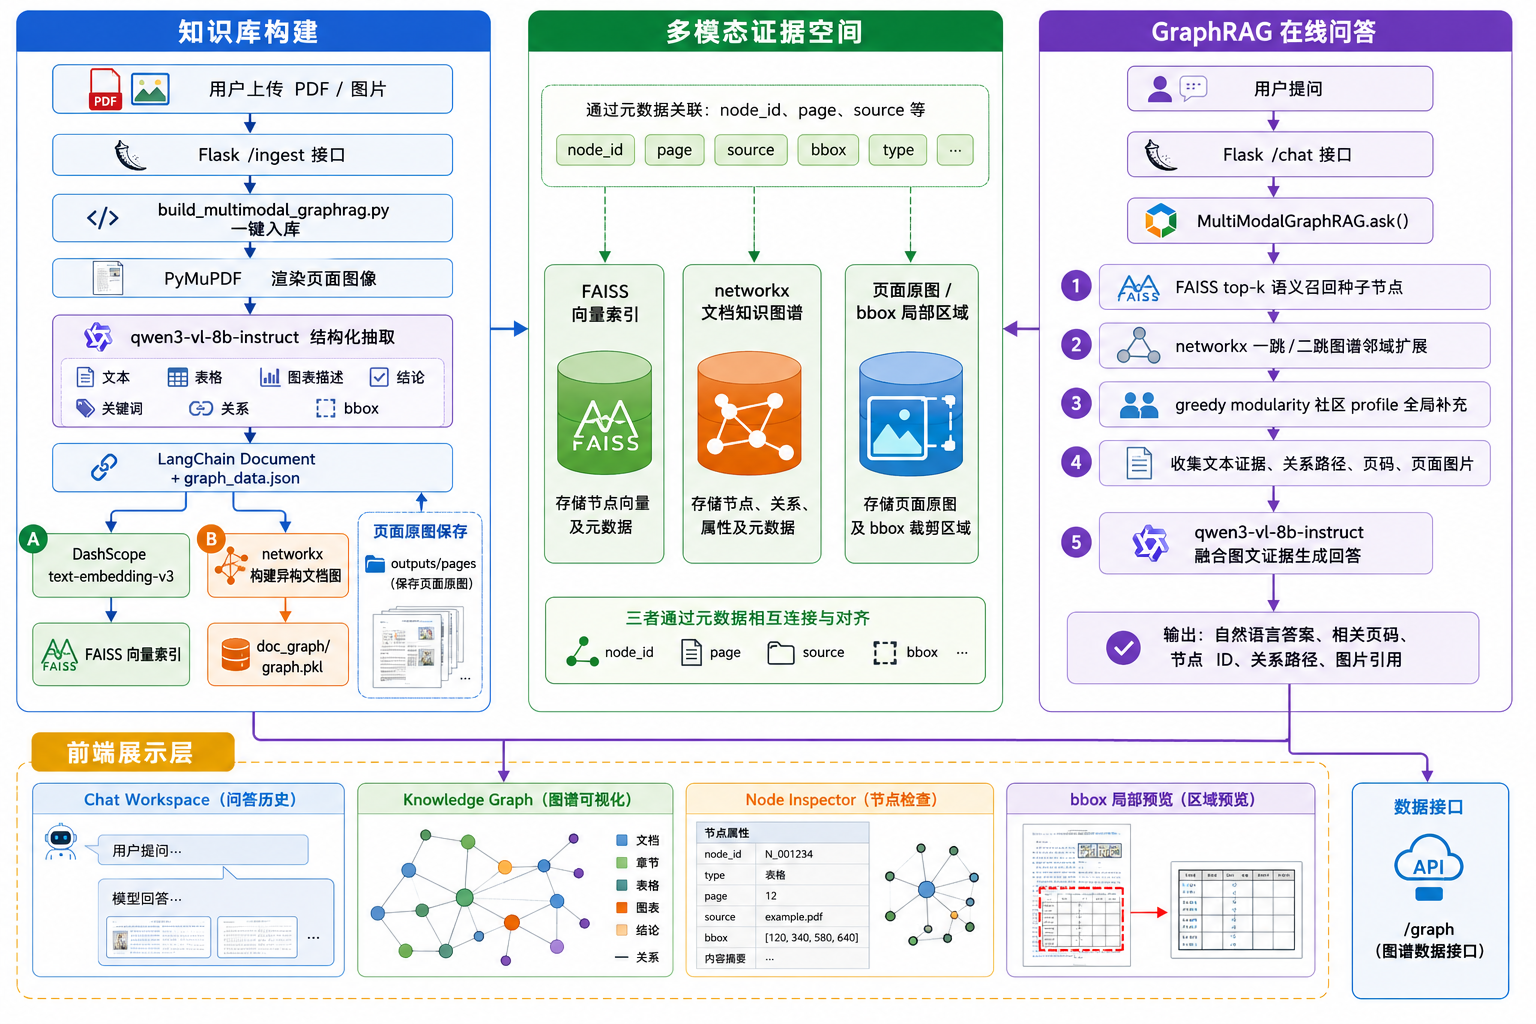
\includegraphics[width=\textwidth,keepaspectratio]{DocRAG架构.png}}
\caption{系统总体架构}
\end{figure}

系统整体围绕``知识库构建''和``在线问答''两条链路展开。知识库构建链路负责把用户上传的多页
PDF 或单页图片转化为可检索、可追溯的多模态证据空间：后端通过 Flask
\texttt{/ingest} 接口接收文件后，调用
\path{build_multimodal_graphrag.py} 执行入库流程。对于 PDF
文件，系统首先使用 PyMuPDF
将每一页渲染为页面图像；对于图片输入，则直接整理为统一的页面图像格式。随后，qwen3-vl-8b-instruct
对页面图像进行结构化抽取，得到文本块、表格、图表描述、页面结论、关键词、关系和
bbox 等信息，并将这些内容封装为 LangChain \texttt{Document}，同时保存为
\texttt{graph\_data.json} 等中间产物。

在知识存储层，系统将同一批结构化内容分别写入向量索引和图谱结构中。一方面，文本、表格、图表描述和结论等内容会通过
DashScope \texttt{text-embedding-v3} 生成向量，并建立本地 FAISS
索引，用于后续的语义召回；另一方面，系统使用 networkx 构建异构文档图，将
text、table、figure、conclusion、cross\_page\_text 和 keyword
等内容组织为节点，并通过
same\_page、keyword\_hit、continuation、cross\_page\_merge 以及 VLM
抽取关系等边连接起来。FAISS 索引、networkx
图谱和页面原图并不是彼此割裂的模块，而是通过
\texttt{node\_id}、\texttt{page}、\texttt{source}、\texttt{image\_path}
和 \texttt{bbox} 等元数据对齐，从而形成统一的多模态证据空间。

在线问答链路从用户问题开始，经由 Flask \texttt{/chat} 接口进入
\texttt{MultiModalGraphRAG.ask()}。系统首先使用 FAISS 对问题进行 top-k
语义召回，得到与问题最相关的种子节点；随后在 networkx
文档图中以这些节点为起点进行一跳邻域扩展，并通过关键词或实体类 hub
做二跳桥接，以补充单次向量检索可能遗漏的上下文。对于更宏观的问题，系统还会基于图结构生成轻量社区
profile，并根据查询词命中、种子节点重叠、社区规模和页码覆盖等因素选择全局补充证据。最终，问答链会收集文本证据、关系路径、相关页码和页面图片，构造包含``图谱关系链
+ 全局社区证据 + 文本证据 + 页面原图''的多模态 prompt，再调用
qwen3-vl-8b-instruct 生成回答。

前端展示层负责把系统的检索与推理过程以更直观的方式呈现出来。Chat
Workspace 展示用户问题和模型回答；Knowledge Graph 使用 vis-network
可视化文档图中的节点和边；Node Inspector 展示节点内容、页码、图像路径和
bbox
局部裁剪预览。这样的设计使系统不仅能够给出自然语言答案，还能返回相关页码、节点
ID、关系路径和页面图像引用，便于在课程演示和错误分析中说明答案来源。

\section{核心模块}\label{ux6838ux5fc3ux6a21ux5757}

\begin{longtable}[]{@{}
  >{\raggedright\arraybackslash}p{(\linewidth - 4\tabcolsep) * \real{0.3333}}
  >{\raggedright\arraybackslash}p{(\linewidth - 4\tabcolsep) * \real{0.3333}}
  >{\raggedright\arraybackslash}p{(\linewidth - 4\tabcolsep) * \real{0.3333}}@{}}
\toprule\noalign{}
\begin{minipage}[b]{\linewidth}\raggedright
模块
\end{minipage} & \begin{minipage}[b]{\linewidth}\raggedright
对应文件
\end{minipage} & \begin{minipage}[b]{\linewidth}\raggedright
已实现功能
\end{minipage} \\
\midrule\noalign{}
\endhead
\bottomrule\noalign{}
\endlastfoot
配置管理 & \path{src/config.py} & 读取 \texttt{.env}，配置 DashScope
API、模型名、文档目录和输出目录 \\
VLM 调用 & \path{src/vl_client.py} & 将页面图片转为 base64 data
URI，调用 DashScope \texttt{MultiModalConversation}，带瞬时错误重试 \\
文档解析 & \path{src/parsing/pipeline.py} & PDF
渲染、图片准备、页面结构化抽取、稀疏结果重试、文本兜底抽取、bbox
归一化 \\
向量入库 & \path{src/indexing/faiss_store.py} & 使用
DashScopeEmbeddings 分批嵌入，构建并保存 FAISS 索引 \\
图谱构建 & \path{src/graph/builder.py} &
构建内容节点、关键词节点、同页边、continuation 边、cross\_page\_merge
边和语义关系边 \\
一键入库 & \path{build_multimodal_graphrag.py} &
文件签名、增量入库、产物复用、文档注册表、FAISS 与图谱重建 \\
GraphRAG 问答 & \path{src/rag/multimodal_graph_rag_chain.py} &
向量召回、图邻域扩展、社区 profile 选择、图文证据融合回答 \\
后端服务 & \path{src/server.py} & Flask
静态前端、上传入库、问答接口、图谱数据接口、输出文件访问 \\
前端界面 & \path{web/index.html}, \path{web/app.js},
\path{web/styles.css} & 上传、聊天、vis-network
图谱可视化、节点检查器和 bbox 局部裁剪预览 \\
评测脚本 & \path{eval/code/*.py} & DocVQA
数据加载、评测知识库构建、ANLS/EM 计算、预测与错误样例保存 \\
\end{longtable}

\section{文档解析与结构化表示}\label{ux6587ux6863ux89e3ux6790ux4e0eux7ed3ux6784ux5316ux8868ux793a}

系统首先使用 PyMuPDF 将 PDF 页面以较高缩放比例渲染为 PNG。随后，解析
prompt 要求 qwen3-vl-8b-instruct 输出统一 JSON：

\begin{itemize}
\tightlist
\item
  \texttt{texts}：正文、标题、图注等文本块；
\item
  \texttt{tables}：表格内容或 Markdown 表格；
\item
  \texttt{figures}：图像/图表编号、描述和 bbox；
\item
  \texttt{section\_conclusions}：页面或小节结论；
\item
  \texttt{keywords}：方法、模型、数据集、指标、任务等高价值名词短语；
\item
  \texttt{relations}：从页面中抽取的三元组关系。
\end{itemize}

解析模块设计了两类鲁棒性策略：第一，若结构化抽取过稀疏，会自动使用更高召回的
repair prompt 重试；第二，若仍缺少文本块，会额外调用 text-only prompt
进行兜底抽取。所有内容片段都会被赋予稳定 \texttt{node\_id}，并保留
\texttt{source}、\texttt{page}、\texttt{type}、\texttt{image\_path}、\texttt{bbox}、\texttt{fig\_id}
等元数据，为检索、引用和前端可视化提供统一索引。

\section{图谱构建}\label{ux56feux8c31ux6784ux5efa}

当前图谱不是传统意义上只包含``实体-关系''的知识库，而是面向文档问答的\textbf{异构文档图}。节点包括：

\begin{itemize}
\tightlist
\item
  内容节点：text、table、figure、conclusion、cross\_page\_text；
\item
  关键词节点：method、model、dataset、metric、task、concept 等；
\item
  页面相关信息：通过页面节点和 \texttt{contains} 关系在前端中展示。
\end{itemize}

边包括：

\begin{itemize}
\tightlist
\item
  \texttt{same\_page}：同一页内容节点之间的局部上下文联系；
\item
  \texttt{keyword\_hit}：关键词与页面内容锚点之间的双向连接；
\item
  \texttt{cooccurrence}：同页关键词之间的共现关系；
\item
  \texttt{continuation}：相邻页面文本延续；
\item
  \texttt{cross\_page\_merge}：跨页合并片段与原始前后节点的联系；
\item
  VLM 抽取关系：例如方法、模型、指标、图表描述之间的语义边。
\end{itemize}

这种设计比``只抽实体''的图谱更贴合文档问答：页面、图表、表格和跨页段落本身就是重要证据节点。系统还故意弱化了不稳定的实体节点，优先使用关键词和内容锚点，以降低同名实体、别名和幻觉关系带来的噪声。

\section{GraphRAG 检索与生成}\label{graphrag-ux68c0ux7d22ux4e0eux751fux6210}

问答链 \texttt{MultiModalGraphRAG.ask()} 的核心步骤如下：

\begin{enumerate}
\def\labelenumi{\arabic{enumi}.}
\tightlist
\item
  使用 FAISS 对用户问题做 top-k 语义召回，得到种子 \texttt{node\_id}；
\item
  在 networkx 图中从种子节点出发扩展一跳邻居，并通过关键词/实体类 hub
  做二跳桥接；
\item
  将图转为无向图后使用 greedy modularity communities 生成社区
  profile，按查询词命中、种子节点重叠、社区规模和页码覆盖选择全局补充证据；
\item
  收集融合后的节点内容、关系路径、页码、页面图片和跨页图片；
\item
  构造包含``图谱关系链 + 全局社区证据 + 文本证据 + 页面原图''的多模态
  prompt；
\item
  调用 qwen3-vl-8b-instruct
  生成回答，并返回答案、页码、节点、关系和图片路径。
\end{enumerate}

这一设计对应微软 GraphRAG 中 local/global
两类思想，但采用更适合课程项目的轻量实现：局部扩展负责具体证据定位，社区
profile 负责补充全局上下文，页面图像负责恢复图表、版面和视觉细节。

\chapter{模型与技术选型}\label{ux56dbux6a21ux578bux4e0eux6280ux672fux9009ux578b}

\begin{longtable}[]{@{}
  >{\raggedright\arraybackslash}p{(\linewidth - 4\tabcolsep) * \real{0.3333}}
  >{\raggedright\arraybackslash}p{(\linewidth - 4\tabcolsep) * \real{0.3333}}
  >{\raggedright\arraybackslash}p{(\linewidth - 4\tabcolsep) * \real{0.3333}}@{}}
\toprule\noalign{}
\begin{minipage}[b]{\linewidth}\raggedright
组件
\end{minipage} & \begin{minipage}[b]{\linewidth}\raggedright
选型
\end{minipage} & \begin{minipage}[b]{\linewidth}\raggedright
理由
\end{minipage} \\
\midrule\noalign{}
\endhead
\bottomrule\noalign{}
\endlastfoot
文档解析与回答模型 & qwen3-vl-8b-instruct & 支持
OCR、文档结构理解、图像问答和较强多模态推理；API 调用降低本地算力压力 \\
多模态 API & DashScope \texttt{MultiModalConversation} & 与 Qwen
系列模型适配，便于课程项目快速联调 \\
文本嵌入 & DashScope \texttt{text-embedding-v3} &
与主模型同平台，支持中英文文档，适合 FAISS 本地索引 \\
向量数据库 & FAISS & 轻量、本地、无需额外服务，适合课程演示和离线评测 \\
图谱库 & networkx & Python
原生体验好，便于构建有向图、邻域扩展和社区发现 \\
文档渲染 & PyMuPDF & CPU 环境即可快速将 PDF 页面转为图片 \\
后端 & Flask & 简洁稳定，方便提供 \texttt{/ingest}、\texttt{/chat} 和
\texttt{/graph} 接口 \\
前端 & 原生 HTML/CSS/JS + vis-network &
便于图谱可视化、节点检查和轻量部署 \\
评测 & 自建脚本 + ANLS/EM & 与 DocVQA
评测习惯兼容，便于保存预测、指标和错误案例 \\
\end{longtable}

\chapter{数据集与实验设计}\label{ux4e94ux6570ux636eux96c6ux4e0eux5b9eux9a8cux8bbeux8ba1}

\section{数据集计划}\label{ux6570ux636eux96c6ux8ba1ux5212}

\begin{enumerate}
\def\labelenumi{\arabic{enumi}.}
\tightlist
\item
  \textbf{自建长文档测试集}：选择 3-5
  篇含图表、表格、跨页段落和结论引用的论文或技术文档，人工编写问题，覆盖文本理解、表格查询、图表解释、跨页证据、多跳推理和引用定位。
\item
  \textbf{DocVQA 子集}：使用公开 DocVQA
  标注中的验证样本，评估系统在单页文档问答上的抽取式准确性，指标使用
  ANLS 与 Exact Match。
\item
  \textbf{ChartQA
  子集}：抽取图表推理问题，用于观察页面原图和图表描述在视觉/逻辑问题中的作用。
\end{enumerate}

\section{评测问题类型}\label{ux8bc4ux6d4bux95eeux9898ux7c7bux578b}

\begin{longtable}[]{@{}
  >{\raggedright\arraybackslash}p{(\linewidth - 4\tabcolsep) * \real{0.3333}}
  >{\raggedright\arraybackslash}p{(\linewidth - 4\tabcolsep) * \real{0.3333}}
  >{\raggedright\arraybackslash}p{(\linewidth - 4\tabcolsep) * \real{0.3333}}@{}}
\toprule\noalign{}
\begin{minipage}[b]{\linewidth}\raggedright
类型
\end{minipage} & \begin{minipage}[b]{\linewidth}\raggedright
目标
\end{minipage} & \begin{minipage}[b]{\linewidth}\raggedright
示例
\end{minipage} \\
\midrule\noalign{}
\endhead
\bottomrule\noalign{}
\endlastfoot
文本定位 & 检查 OCR/文本抽取和语义召回能力 & ``第 3
节提出的方法核心思想是什么？'' \\
表格问答 & 检查表格抽取和结构理解 & ``表 2 中哪个模型在 DocVQA
上得分最高？'' \\
图表理解 & 检查 VLM 对页面图像和图表描述的利用 & ``图 4
展示了什么趋势？'' \\
跨页延续 & 检查 \texttt{cross\_page\_text} 与 \texttt{continuation} 边 &
``第 1 页末尾延续到第 2 页的段落主要讲什么？'' \\
多跳关系 & 检查图谱扩展是否能补足单次向量召回 &
``某方法的结论由哪些图表或实验结果支撑？'' \\
引用追踪 & 检查答案是否能给出页码、图号和关系依据 &
``请回答并标出相关页码和关键节点。'' \\
\end{longtable}

\section{指标设计}\label{ux6307ux6807ux8bbeux8ba1}

\begin{longtable}[]{@{}
  >{\raggedright\arraybackslash}p{(\linewidth - 4\tabcolsep) * \real{0.3333}}
  >{\raggedright\arraybackslash}p{(\linewidth - 4\tabcolsep) * \real{0.3333}}
  >{\raggedright\arraybackslash}p{(\linewidth - 4\tabcolsep) * \real{0.3333}}@{}}
\toprule\noalign{}
\begin{minipage}[b]{\linewidth}\raggedright
指标
\end{minipage} & \begin{minipage}[b]{\linewidth}\raggedright
说明
\end{minipage} & \begin{minipage}[b]{\linewidth}\raggedright
适用范围
\end{minipage} \\
\midrule\noalign{}
\endhead
\bottomrule\noalign{}
\endlastfoot
ANLS & 平均归一化编辑相似度，DocVQA 常用指标 & DocVQA/短答案问题 \\
Exact Match & 预测答案与任一标准答案完全匹配 & DocVQA/短答案问题 \\
人工准确率 & 三档评分：正确、部分正确、错误 & 自建长文档问题 \\
引用命中率 & 回答给出的页码、图号、节点是否覆盖真实证据 &
自建问题与案例分析 \\
证据召回率 & top-k + 图扩展后的证据中是否包含人工标注依据 &
自建可标注问题 \\
图谱有效性 & 开启/关闭图扩展时多跳题表现差异 & 消融实验 \\
运行代价 & 入库耗时、问答耗时、API 调用次数和 token 成本 & 工程可行性 \\
\end{longtable}

\chapter{算力预算与时间计划}\label{ux516dux7b97ux529bux9884ux7b97ux4e0eux65f6ux95f4ux8ba1ux5212}

\section{算力与成本}\label{ux7b97ux529bux4e0eux6210ux672c}

\begin{longtable}[]{@{}
  >{\raggedright\arraybackslash}p{(\linewidth - 4\tabcolsep) * \real{0.3333}}
  >{\raggedright\arraybackslash}p{(\linewidth - 4\tabcolsep) * \real{0.3333}}
  >{\raggedright\arraybackslash}p{(\linewidth - 4\tabcolsep) * \real{0.3333}}@{}}
\toprule\noalign{}
\begin{minipage}[b]{\linewidth}\raggedright
资源
\end{minipage} & \begin{minipage}[b]{\linewidth}\raggedright
需求
\end{minipage} & \begin{minipage}[b]{\linewidth}\raggedright
方案
\end{minipage} \\
\midrule\noalign{}
\endhead
\bottomrule\noalign{}
\endlastfoot
本地计算 & CPU 即可 & PDF 渲染、FAISS、networkx 和 Flask 均可本地运行 \\
GPU & 非必需 & 使用 DashScope API 调用 qwen3-vl-8b-instruct \\
存储 & 百 MB 到数 GB & 页面图片、FAISS 索引、JSON
解析结果和图谱文件保存在 \texttt{outputs/} 或 \texttt{eval/output/} \\
API 成本 & 与页数和问题数相关 & 先小样本评测，再扩展；复用 build meta
避免重复入库 \\
网络 & 构建和问答时需要 & API
调用依赖外部服务；本地检索与图谱读取不依赖网络 \\
\end{longtable}

\section{当前进度}\label{ux5f53ux524dux8fdbux5ea6}

\begin{longtable}[]{@{}
  >{\raggedright\arraybackslash}p{(\linewidth - 4\tabcolsep) * \real{0.3333}}
  >{\raggedright\arraybackslash}p{(\linewidth - 4\tabcolsep) * \real{0.3333}}
  >{\raggedright\arraybackslash}p{(\linewidth - 4\tabcolsep) * \real{0.3333}}@{}}
\toprule\noalign{}
\begin{minipage}[b]{\linewidth}\raggedright
阶段
\end{minipage} & \begin{minipage}[b]{\linewidth}\raggedright
状态
\end{minipage} & \begin{minipage}[b]{\linewidth}\raggedright
产出
\end{minipage} \\
\midrule\noalign{}
\endhead
\bottomrule\noalign{}
\endlastfoot
工程骨架 & 已完成 &
\texttt{src/}、\texttt{web/}、\texttt{eval/}、\texttt{requirements.txt}、运行说明 \\
文档解析 & 已完成初版 & VLM JSON 抽取、bbox、重试和文本兜底 \\
向量索引 & 已完成 & FAISS 本地索引与增量重建 \\
图谱构建 & 已完成初版 & networkx
文档图、关键词节点、跨页边、同页边、关系边 \\
GraphRAG 问答 & 已完成初版 & 向量召回 + 图扩展 + 社区 profile +
页面图像生成 \\
Web 演示 & 已完成初版 & 上传入库、聊天、图谱可视化、节点检查 \\
评测脚本 & 已完成框架 & DocVQA KB 构建、ANLS/EM、预测与错误样例输出 \\
\end{longtable}

\section{后续计划}\label{ux540eux7eedux8ba1ux5212}

\begin{longtable}[]{@{}
  >{\raggedright\arraybackslash}p{(\linewidth - 4\tabcolsep) * \real{0.3333}}
  >{\raggedright\arraybackslash}p{(\linewidth - 4\tabcolsep) * \real{0.3333}}
  >{\raggedright\arraybackslash}p{(\linewidth - 4\tabcolsep) * \real{0.3333}}@{}}
\toprule\noalign{}
\begin{minipage}[b]{\linewidth}\raggedright
时间
\end{minipage} & \begin{minipage}[b]{\linewidth}\raggedright
工作
\end{minipage} & \begin{minipage}[b]{\linewidth}\raggedright
产出
\end{minipage} \\
\midrule\noalign{}
\endhead
\bottomrule\noalign{}
\endlastfoot
第 1 周 & 清理图谱噪声、优化关键词和关系过滤 & 更稳定的
\texttt{graph\_data.json} 与图谱统计 \\
第 2 周 & 构建自建长文档测试集，补充 DocVQA 小样本 &
\path{test_questions.json}、评测输入 \\
第 3 周 & 跑 Full/No-Graph/No-Image 消融实验 &
指标表、错误案例、运行成本记录 \\
第 4 周 & 完善前端演示、整理最终报告和答辩材料 & Demo
视频、最终报告、展示 PPT \\
\end{longtable}

\chapter{创新点与贡献}\label{ux516bux521bux65b0ux70b9ux4e0eux8d21ux732e}

\begin{enumerate}
\def\labelenumi{\arabic{enumi}.}
\tightlist
\item
  \textbf{以 GraphRAG
  作为主线而非附加模块}：从入库开始同时构建向量索引和文档图谱，使文本、图表、页面和跨页关系处于同一证据空间。
\item
  \textbf{页面图像驱动的结构化解析}：直接使用 VLM
  从页面图像中抽取文本、表格、图表、结论、关键词和关系，减少传统 OCR +
  版面规则流水线的复杂度。
\item
  \textbf{面向文档的异构图设计}：把
  text/table/figure/conclusion/cross\_page\_text 和 keyword
  都纳入图谱，而不局限于传统实体关系图。
\item
  \textbf{向量检索与图谱扩展融合}：先用 FAISS 找到语义种子，再用
  networkx 邻域和社区 profile
  扩展证据，兼顾具体证据定位和全局上下文补充。
\item
  \textbf{可解释前端展示}：前端不仅返回答案，还展示图谱节点、边、页码、bbox
  局部图像和关系路径，便于课程演示和错误分析。
\item
  \textbf{低资源可落地}：无需本地 GPU，核心计算依赖轻量本地组件和 API
  调用，适合课程项目周期内完成。
\end{enumerate}

\chapter{参考文献}\label{ux53c2ux8003ux6587ux732e}

{[}1{]} Lewis, P. et al.~(2020). Retrieval-Augmented Generation for
Knowledge-Intensive NLP Tasks. NeurIPS 2020.
\url{https://papers.nips.cc/paper_files/paper/2020/hash/6b493230205f780e1bc26945df7481e5-Abstract.html}

{[}2{]} Edge, D. et al.~(2024). From Local to Global: A Graph RAG
Approach to Query-Focused Summarization. arXiv:2404.16130.
\url{https://graphrag.com/appendices/research/2404.16130/}

{[}3{]} Microsoft GraphRAG Documentation. Query Engine Overview and
Indexing Overview. \url{https://microsoft.github.io/graphrag/query/overview/}
; \url{https://microsoft.github.io/graphrag/index/overview/}

{[}4{]} Mathew, M., Karatzas, D., Jawahar, C. V. (2021). DocVQA: A
Dataset for VQA on Document Images. WACV 2021.
\url{https://site.docvqa.org/datasets/docvqa}

{[}5{]} Masry, A. et al.~(2022). ChartQA: A Benchmark for Question
Answering about Charts with Visual and Logical Reasoning. Findings of
ACL 2022. \url{https://aclanthology.org/2022.findings-acl.177/}

{[}6{]} Faysse, M. et al.~(2024). ColPali: Efficient Document Retrieval
with Vision Language Models. arXiv:2407.01449.
\url{https://huggingface.co/papers/2407.01449}

{[}7{]} Qwen Team. Qwen3-VL official repository and Qwen3-VL-8B-Instruct
model card. \url{https://github.com/QwenLM/Qwen3-VL} ;
\url{https://huggingface.co/Qwen/Qwen3-VL-8B-Instruct}

{[}8{]} Dong, K. et al.~(2025). Benchmarking Retrieval-Augmented
Multimodal Generation for Document Question Answering. MMDocRAG.
\url{https://mmdocrag.github.io/MMDocRAG/}

{[}9{]} Bu, C. et al.~(2025). Query-Driven Multimodal GraphRAG: Dynamic
Local Knowledge Graph Construction for Online Reasoning. Findings of ACL
2025. \url{https://aclanthology.org/2025.findings-acl.1100/}
